
\documentclass[a4paper,10pt,reqno]{amsart}

\usepackage[T1]{fontenc}

\usepackage[bitstream-charter]{mathdesign}
\usepackage{tgheros}  %  the advanced helvet as it was nice.



% Redefine cite so that we get references in footnotes.
\usepackage[
backend=biber,
citestyle=authoryear,
bibstyle=authoryear,
sorting=none,
firstinits=true,
maxcitenames=2
]{biblatex} %style=mla for footnotes.
%\renewcommand{\cite}[1]{\footcite{#1}}
\renewcommand{\cite}[1]{\parencite{#1}}

\addbibresource{epilit.bib}


% This has to go below fontenc for some reason
% These lines of code are generated by knitting a .Rtex file.
% We include them here so that we can knit each chapter seperately.
% 

\usepackage{subfig}
\usepackage{color}


%% maxwidth is the original width if it is less than linewidth
%% otherwise use linewidth (to make sure the graphics do not exceed the margin)
\makeatletter
\def\maxwidth{ %
  \ifdim\Gin@nat@width>\linewidth
    \linewidth
  \else
    \Gin@nat@width
  \fi
}
\makeatother

\definecolor{fgcolor}{rgb}{0.345, 0.345, 0.345}
\newcommand{\hlnum}[1]{\textcolor[rgb]{0.686,0.059,0.569}{#1}}%
\newcommand{\hlstr}[1]{\textcolor[rgb]{0.192,0.494,0.8}{#1}}%
\newcommand{\hlcom}[1]{\textcolor[rgb]{0.678,0.584,0.686}{\textit{#1}}}%
\newcommand{\hlopt}[1]{\textcolor[rgb]{0,0,0}{#1}}%
\newcommand{\hlstd}[1]{\textcolor[rgb]{0.345,0.345,0.345}{#1}}%
\newcommand{\hlkwa}[1]{\textcolor[rgb]{0.161,0.373,0.58}{\textbf{#1}}}%
\newcommand{\hlkwb}[1]{\textcolor[rgb]{0.69,0.353,0.396}{#1}}%
\newcommand{\hlkwc}[1]{\textcolor[rgb]{0.333,0.667,0.333}{#1}}%
\newcommand{\hlkwd}[1]{\textcolor[rgb]{0.737,0.353,0.396}{\textbf{#1}}}%

\usepackage{framed}
\makeatletter
\newenvironment{kframe}{%
 \def\at@end@of@kframe{}%
 \ifinner\ifhmode%
  \def\at@end@of@kframe{\end{minipage}}%
  \begin{minipage}{\columnwidth}%
 \fi\fi%
 \def\FrameCommand##1{\hskip\@totalleftmargin \hskip-\fboxsep
 \colorbox{shadecolor}{##1}\hskip-\fboxsep
     % There is no \\@totalrightmargin, so:
     \hskip-\linewidth \hskip-\@totalleftmargin \hskip\columnwidth}%
 \MakeFramed {\advance\hsize-\width
   \@totalleftmargin\z@ \linewidth\hsize
   \@setminipage}}%
 {\par\unskip\endMakeFramed%
 \at@end@of@kframe}
\makeatother

\definecolor{shadecolor}{rgb}{.97, .97, .97}
\definecolor{messagecolor}{rgb}{0, 0, 0}
\definecolor{warningcolor}{rgb}{1, 0, 1}
\definecolor{errorcolor}{rgb}{1, 0, 0}
\newenvironment{knitrout}{}{} % an empty environment to be redefined in TeX

\usepackage{alltt}
\IfFileExists{upquote.sty}{\usepackage{upquote}}{}




\usepackage{caption}
\usepackage{verbatim, geometry, fancyhdr,  graphicx, xcomment, microtype, array}
%\usepackage{amsmath}



\usepackage{booktabs}
\usepackage[pdftex,hidelinks]{hyperref}



% Setup environment `entry' to use `entry*' with a drop cap
\newcommand{\lettr}[1]{#1}
% Setup environment `entry*' so that lettrine can be manually specified if needed

\newcommand{\tmpsection}[1]{\subsubsection{#1}}





\setcounter{tocdepth}{4} % make TOC go to subsubsection



\begin{document}


\title{The interactions between population structure and density in pathogen diversity}
\author{Tim Lucas. \today}
\date{}

\maketitle
%\tableofcontents












\section{Abstract}


\tmpsection{One or two sentences providing a basic introduction to the field}
% comprehensible to a scientist in any discipline.
\lettr{A}n increasingly large fraction of emerging diseases come from animals \cite{jones2008global, taylor2001risk} and these diseases have a huge impact on human health.
The chance that a new disease will come from any particularly wild host species increases with the diversity of pathogens in that species.
However, the factors that control pathogen diversity in wild populations are still unknown.



\tmpsection{Two to three sentences of more detailed background}
Population density is known to increase pathogen richness while theory suggests that population structure may also play a role.
However, these factors, along with population abundance, are intrinsically linked; reducing density reduces contacts between individuals.
In group living species, this is particularly true, with group size and the number of groups and distribution size contributing to total animal density. 
As these factors are completely interdependant, it is very difficult to study them empirically e.g. in a comparative frame work.

\tmpsection{One sentence clearly stating the general problem (the gap)}
% being addressed by this particular study.

It is unknown whether it is specifically density that controls pathogen diversity or whether density merely correlates with population structure, group size or population size (abundance).


\tmpsection{One sentence summarising the main result}
%  (with the words “here we show” or their equivalent).
Here I use metapopulation SIR models to test whether it is density \emph{per se} that increases the ability of a new pathogen to invade as apposed to colony size, population abundance or population structure.



\tmpsection{Two or three sentences explaining what the main result reveals in direct comparison to what was thought to be the case previously}
% or how the main result adds to previous knowledge



\tmpsection{One or two sentences to put the results into a more general context.}

\tmpsection{Two or three sentences to provide a broader perspective, }
% readily comprehensible to a scientist in any discipline.





%%%%%%%%%%%%%%%%%%%%%%%%%%%%%%%%%%%%%%%%%%%%%%%%%%%%%%%%%%%%%%%%%%%%%%%%%%%%%%%%%%%%%%%%%%%%%%%%%%%%%%%%%%%%%%%%%%%%%%%%%%%%%%%%%%%%%%%%%%%%%%%%%%%%%%%%%%%


\section{Introduction}

%%%%%%%%%%%%%%%%%%%%%%%%%%%%%%%%%%%%%%%%%%%%%%%%%%%%%%%%%%%%%%%%%%%%%%%%%%%%%%%%%%%%%%%%%%%%%%%%%%%%%%%%%%%%%%%%%%%%%%%%%%%%%%%%%%%%%%%%%%%%%%%%%%%%%%%%%%%




\tmpsection{General Intro}
%%%%%%%%%%%%%%%%%%%%%%%%%%%%%%
% A basic introduction to the field,
% comprehensible to a scientist in any discipline.

Zoonotic diseases are an increasingly important source of human infectious diseases \cite{jones2008global, woolhouse2006host, taylor2001risk}.
The diversity of pathogens in wild animal populations is huge and largely unknown \cite{poulin2014parasite}.
The factors that allow large numbers of pathogen species to coexist in a host \cite{anthony2013strategy, anthony2013strategy} are still unclear.
It is likely that population level factors such as population density, range size and population structure have an important role in controlling pathogen community dynamics.
Global change is strongly peturbing wild animal populations, but without clear mechanistic models of how these populations maintain pathogen species richness, we can not predict how pathogen communities, and the risks of zoonotic outbreaks, will change in the coming decades.





\tmpsection{Specific Intro}
%%%%%%%%%%%%%%%%%%%%%%%%%%%%%%
% more detailed background}
% comprehensible to scientists in related disciplines.

\tmpsection{Theoretical background}
Variables that describe populations, such as population density and structure, are well established as having a central role in pathogen dynamics \cite{colizza2007invasion, barthelemy2010fluctuation, colizza2007invasion,  wu2013threshold, may1979population, anderson1979population}.
More recently, the role of the population has been examined with respect to pathogen richness and the coexistence of competing pathogens \cite{qiu2013vector, allen2004sis, nunes2006localized}.
Yet even in theoretical studies there is confusion as to how exactly we should measure populations.
There is disagreement on whether population density (individuals per unit area) should be preferred over population abundance (number of individuals) \cite{begon2002clarification} and how exactly area should be incorporated \cite{begon2002clarification}. 


\tmpsection{Density/abundance in comparative research}
With the increase of novel zoonotic pathogens \cite{} attention has turned to comparatively assessing the factors that are associated with high or low pathogen richness in wild animal species \cite{morand review}.
Here again there is little clarity on the relationship between a number of species measurements.
Population density is commonly studied \cite{} as is range size \cite{}.
However it is rarely if ever acknowledge that these two values are intrinsically linked by $d = N/a$ where $d$ is density, $N$ is the population size and $a$ is area.
In contrast, abundance has never been directly studied as a predictor of pathogen richness.
This is  a glaring omission as abundance more closely aligns with the ``island-biogeography'' class of mechanisms posited to explain pathogen richness \cite{}.
Furthermore, abundance is considered the more relevant measure in terms of pathogen dynamics, especially when area cannot be assumed to be constant \cite{begon} as is commonly the case in wild populations, especially in the face of global warming and habitat degradation.

\tmpsection{Populatiion structure in comparative research}
It is clear that individuals of an animal species are not randomly distributed in space: social groups are common \cite{} and geographic boundaries reduce contacts between isolated populations.
In social species, measures such as global population density are largely meaningless with respect to the number of infectious contacts individuals may have.
Rather, contacts are based on group size and rates of movements between groups.
Two aspects of non-random transmission have been studied in particular: group size \cite{nunn and others} and global measures of population structure including genetic measures and measures derived from distribution shapes (\textcite{gay, maganga, turmelle} and see Chapter \ref{ch:}).
Again however, the relationships between these terms and more the more global terms mentioned above are rarely examined.
Population abundance can be decomposed into two components, the number of groups and the average size of a group with $N = nm$ where $n$ is group size and $m$ is the number of groups.
The amount of movement between is largely dependant on the distance between groups.
This depends on the number of groups per area $m/a$ or $N/na$ and the average distance between groups, if groups are randomly distributed in space scales as $something$.

\tmpsection{But reaction to climate change, and predictions depend on which factor is actually important}


Importantly, these factors, although interrelated, will respond differently to global change and the response will be species dependant.
Some species may suffer large range contractions, and therefore large falls in absolute abundance, while their density remains fairly constant.
Other species might be expected to retain their distribution but have a depressed population density across their range.
Similarly with population structure, species particularly affected by habitat fragmentation can expect increased reduced movement of individuals between groups, while other species may be most affected by a reduction in group size.
Furthermore, different mechanisms of maintenance and creation of pathogen richness will respond to changes in these factors differently as well.
If pathogen richness ultimately depends on the ``island size'' of the host population, then falls in population abundance will reduce pathogen richness the most.
If local group size affects the ability of new pathogens to invade (Chapter \ref{ch:sim1}) then changes in group size are likely to be most important.
Finally, if increased population structure allows pathogens to coexist (\parencite{qiu2013vector, allen2004sis, nunes2006localized} and Chapter \ref{ch:}) increase habitat fragmentation could be expected to increase pathogen richness.

As these factors are likely to be correlated, correlative comparative studies will struggle to distinguish between them.
Furthermore, even if factors are supported or rejected, the specific mechanisms by which the promote pathogen richness will remain unknown, and these may suggest different responses to global change.
Furthermore, mechanistic models are expected to be more predictive into the future and into hitherto unseen parameter space.




\tmpsection{The gap}
%%%%%%%%%%%%%%%%%%%%%%%%%%%%%%

Therefore there is great need to mechanistic models that try to disentangle the interplay between these many factors: density, abundance, range size, population structure, group size and the number of groups.

\tmpsection{What I did and found}
%%%%%%%%%%%%%%%%%%%%%%%%%%%%%%


% One sentence summarising the main result
% (with the words “here we show” or their equivalent).








%%%%%%%%%%%%%%%%%%%%%%%%%%%%%%%%%%%%%%%%%%%%%%%%%%%%%%%%%%%%%%%%%%%%%%%%%%%%%%%%%%%%%%%%%
%%%% Constant density size. 
%%%%%%%%%%%%%%%%%%%%%%%%%%%%%%%%%%%%%%%%%%%%%%%%%%%%%%%%%%%%%%%%%%%%%%%%%%%%%%%%%%%%%%%%%







%%%%%%%%%%%%%%%%%%%%%%%%%%%%%%%%%%%%%%%%%%%%%%%%%%%%%%%%%%%%%%%%%%%%%%%%%%%%%%%%%%%%%%%%%
%%%% Constant density 2. 
%%%%%%%%%%%%%%%%%%%%%%%%%%%%%%%%%%%%%%%%%%%%%%%%%%%%%%%%%%%%%%%%%%%%%%%%%%%%%%%%%%%%%%%%%









%%%%%%%%%%%%%%%%%%%%%%%%%%%%%%%%%%%%%%%%%%%%%%%%%%%%%%%%%%%%%%%%%%%%%%%%%%%%%%%%%%%%%%%%%
%%%% Constant Population. 
%%%%%%%%%%%%%%%%%%%%%%%%%%%%%%%%%%%%%%%%%%%%%%%%%%%%%%%%%%%%%%%%%%%%%%%%%%%%%%%%%%%%%%%%%








\begin{knitrout}\footnotesize
\definecolor{shadecolor}{rgb}{0.969, 0.969, 0.969}\color{fgcolor}\begin{figure}[t]

{\centering 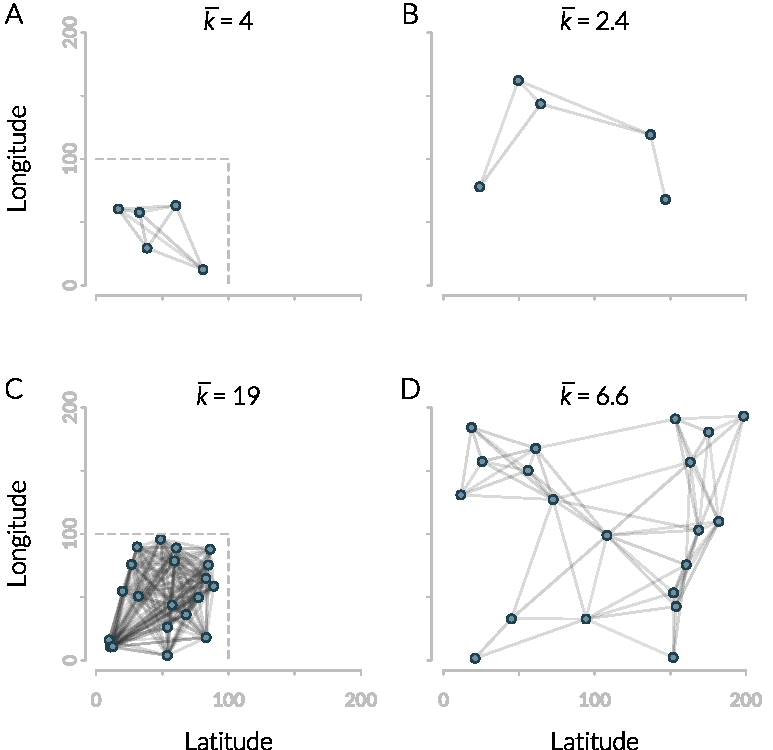
\includegraphics[width=0.9\textwidth]{figure/colonyNetworkPlots-1} 

}

\caption[Example metapopulation networks]{
Examples of the metapopulation networks used.
They show the smallest number of colonies (five) and the default (20).
They also show the default ($10^4\,\text{km}^2$, grey dashed lines) and largest areas ($4\times10^4\,\text{km}^2$, full plot), though all networks are plotted on the largest area.
As area increases, the number of connections each subpopulation has decreases as seen by the changes in mean degree, $\bar{k}$.
}\label{fig:colonyNetworkPlots}
\end{figure}


\end{knitrout}




%%%%%%%%%%%%%%%%%%%%%%%%%%%%%%%%%%%%%%%%%%%%%%%%%%%%%%%%%%%%%%%%%%%%%%%%%%%%%%%%%%%%%%%%%%%%%%%%%%%%%%%%%%%%%%%%%%%%%%%%%%%%%%%%%%%%%%%%%%%%%%%%%%%%%%%%%%%


\section{Methods}

%%%%%%%%%%%%%%%%%%%%%%%%%%%%%%%%%%%%%%%%%%%%%%%%%%%%%%%%%%%%%%%%%%%%%%%%%%%%%%%%%%%%%%%%%%%%%%%%%%%%%%%%%%%%%%%%%%%%%%%%%%%%%%%%%%%%%%%%%%%%%%%%%%%%%%%%%%%

%%




\subsection{Metapopulation model}

\tmpsection{Overview}


I used two-pathogen, metapopulation SIR model to compare the roles of demograhic parameters on pathogen species richness.
Specifically I let two identical pathogens (and endemic pathogen and an invading pathogen) compete.
I used presistence or not of the second pathogen as my response variable.
I test whether population abundance is more important than population density.
I then test whether colony size or the number of colonies is the more important component of population abundance.
The multpathogen SIR model is identical to that in Chapter \ref{ch:sims1} and is implemented in R \cite{R}.



In each simulation the population is seeded with 20 individuals infected with pathogen 1 in each colony. 
Pathogen 1 is then allowed to spread and reach equilibrium. 
After \ensuremath{7\times 10^{5}} events, 5 individuals infected with pathogen 2 are added to one colony. 
After another \ensuremath{3\times 10^{5}} events the invasion of pathogen 2 is considered successful if any individuals with pathogen 2 still remain.

\subsection{Dependant variables}

Three dependant variables were varied: colony size, number of colonies and area.
From these parameters, population abundance and population density can be calculated.
The default values of these parameters was a population size of 8000 individuals split into 20 colonies of 400.
The default area of the simulations was 

Three sets of simulations were run.
First, colony size was varied using values 100, 200, 400, 800 and \ensuremath{1.6\times 10^{3}}.
The number of colonies was kept constant and so population abundance varied with colony size.
Area was scaled to keep population density constant. 
Secondly, number of colonies (and therefore population abundance) was varied and again area was varied to keep density constant.
5, 10, 20, 40 and 80 colonies were used.
Finally, colony size and number of colonies were kept constant (therefore keeping population abundance constant) and area was varied alone to alter population density. 
The values of area used were \ensuremath{4\times 10^{4}}, \ensuremath{2\times 10^{4}}, \ensuremath{10^{4}}, \ensuremath{5\times 10^{3}} and \ensuremath{2.5\times 10^{3}} which gave density values of 0.2, 0.4, 0.8, 1.6 and 3.2.

The affects of area occur through changing the metapopulation network.
The metapopulation structure was created for each simulation by randomly placing colonies in space.
The spatial scale of the simulations vary between \ensuremath{2.5\times 10^{3}} and \ensuremath{4\times 10^{4}} km$^2$ (space is given in kilometers even though they are oin fact arbitrary units for simplicity).
This corresponds to square areas with sides of 50 to 200 km).
Dispersal can only occur between two colonies if they are within 100 kilometers of each other i.e. they are connected nodes in the metapopulation network.
The number of connections each colony has is called its degree, $k$.
How well connected the metapopulation network is overall is measured by the mean degree, $\bar{k}$.
This does not guarentee that the population is fully connected but as the endemic pathogen is seeded in all colonies, the invading pathogen cannot be seeded into a fully susceptible colony.
This was considered more realistic than repeatedly resampling the population until a fully connected population occured.
Given this setup, simulations with low densities had relatively unconnected metapopulation networks.






\subsection{Other Parameters}
%TODO switch all b's to d or something else, so that b can be used for regression coeficients. In all eqns in +ch2 as well.

The fixed parameters used are chosen to roughly reflect realistic wild bat populations. 
The death rate $\Lambda$ is set as 0.05 per year giving a generation time of 20 years.
The birth rate is set to be equal to $\mu$ so that the population size is stable.
The recovery rate $\gamma$ is set to 1 giving a average infection duration of 1 years. 
This is therefore a long lasting infection but not a chronic infection. 
It is very difficult to directly estimate infection durations in wild populations but it seems that these infections might sometimes be long lasting \cite{peel2012henipavirus, plowright2015ecological}.
However, other studies have found much shorter infectious periods \cite{amengual2007temporal}.
These shorter lived in infections are studied further here as preliminary simulations found that they could not persist in the relatively small populations being modelled here.

Cross immunity is set to 0.1 so that an individual infected with one pathogen is 90\% less likely to be infected with another.
This is a rather arbitrary value.
However, the rationale of the model is that the invading species might be a newly speciated strain of the endemic species.
Furthermore, the model assumes complete cross immunity after recovery from infection.
Therefore cross immunity to coinfection is likely to be very strong as well.


The population size of each subpopulation is set to 3,000. 
This is appropriate for many bat species \cite{jones2009pantheria}, especially the large, frugivorous \emph{Pteropodidae} that have been particularly associated with recent zoonotic diseases.


Three values of the transmission rate $\beta$ are used, 0.1, 0.2 and 0.3.
All simulations are run under all three transmission rates as this is a fundamental parameter that changes the broad dynamics of the pathogens.


\subsection{Statistical comparisons}

I tested two hypotheses.
Firstly I tested the hypothesis that an increase in population abundance creates a stronger increase in invasion probability (of the second pathogen) than an equal increase in population density.
Secondly I tested the hypothesis that ana increase in colony size creates a stronger increase in invasion probability an an equal increase in number of colonies.
To statistically test these hypotheses I combined the results from different simulations and fitted multiple logistic regressions, centering and scaling the dependant variables.
Specifically, I fitted the model $\text{invasion} = b_1 \text{density} + b_2 \text{colony size} + b_3 \text{number of colonies} + c + \epsilon$ where $c$ is a fitted intercept and $\epsilon$ is a binomially distributed error term.
To test the first hypothesis I compared the size (and 95\% confidence intervals) of $b_1$ to $b_2$ and $b_3$.
To test the second hypothesis I compared $b_2$ to $b_3$.








%%%%%%%%%%%%%%%%%%%%%%%%%%%%%%%%%%%%%%%%%%%%%%%%%%%%%%%%%%%%%%%%%%%%%%%%%%%%%%%%%%%%%%%%%%%%%%%%%%%%%%%%%%%%%%%%%%%%%%%%%%%%%%%%%%%%%%%%%%%%%%%%%%%%%%%%%%%


\section{Results}

%%%%%%%%%%%%%%%%%%%%%%%%%%%%%%%%%%%%%%%%%%%%%%%%%%%%%%%%%%%%%%%%%%%%%%%%%%%%%%%%%%%%%%%%%%%%%%%%%%%%%%%%%%%%%%%%%%%%%%%%%%%%%%%%%%%%%%%%%%%%%%%%%%%%%%%%%%%






















\begin{knitrout}\footnotesize
\definecolor{shadecolor}{rgb}{0.969, 0.969, 0.969}\color{fgcolor}\begin{figure}[t]

{\centering 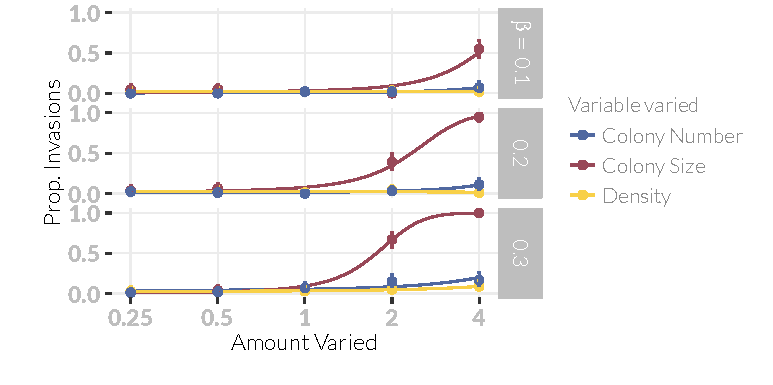
\includegraphics[width=\textwidth]{figure/plotValueChangeMeans-1} 

}

\caption[Comparison of the probability of invasion when population size is altered by changing colony size or colony number.]{
Comparison of the effect of colony size, colony number and area on probability of invasion.
Default values are: colony number = 20, colony size = 400 and density = 0.8 animals per unit area.
The $x$-axis shows the relative change in each of these values ($\times 0.25, 0.5, 1, 2$ and $4$).
For colony size and number, area is altered  so that density remains constant.
For density, population size is constant at 8,000 and area is altered.
Relationships are shown seperately for each transmission value.
Each point is the mean of 
inline{each} simulations and bars are 95\% confidence intervals.
}\label{fig:plotValueChangeMeans}
\end{figure}


\end{knitrout}





\begin{knitrout}\footnotesize
\definecolor{shadecolor}{rgb}{0.969, 0.969, 0.969}\color{fgcolor}\begin{figure}[t]

{\centering 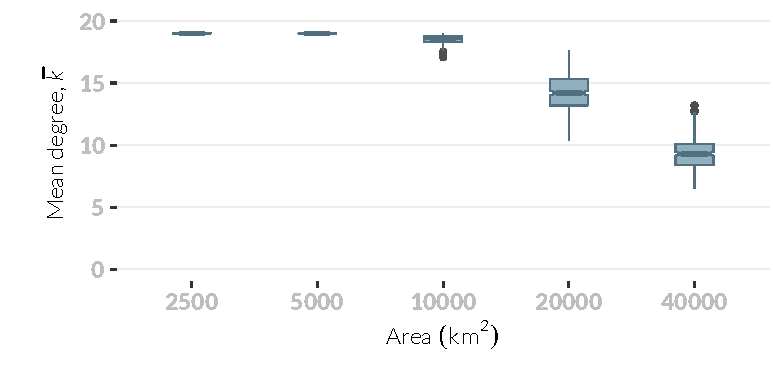
\includegraphics[width=0.8\textwidth]{figure/plotK-1} 

}

\caption[Change in average network degree with increasing area]{
Change in average metapopulation network degree ($\bar{k}$) with increasing area. 
Bars show the median, boxes show the interquartile range, vertical lines show and range and grey dots indicate outlier values.
Notches indicate the 95\% confidence interval of the mean.
}\label{fig:plotK}
\end{figure}


\end{knitrout}





\begin{table}

\caption[Regression results]{
Regression results comparing affects of colony size, colony number and area.
Coefficients are from multiple logistic regressions with invasion as the dependant variable and all independant variables being scaled and centred.
Colony size and colony number were varied while keeping density equal while density was varied by changing area while keeping population size equal.
$p$ is for test against the null hypothesis that  $b = 0$.
}
\label{t:regrCoefs}
\centering
\begin{tabular}{@{}rlrrr@{}}
\toprule
$\beta$ & \emph{Variable} & \emph{Estimate} ($b$) & (95\% \emph{CI}) & $p$\\
\midrule
0.1   &    Intercept     & \ensuremath{-3.52} & (\ensuremath{-3.87}, \ensuremath{-3.2}) & $< 10^{-5}$ \\
      &    Colony Size   & 1.07 & (0.75, 1.49) & $< 10^{-5}$ \\
      &    Colony Number & 0.35 & (\ensuremath{-0.02}, 0.79) & 0.08 \\
      &    Density       & 0.01 & (\ensuremath{-0.66}, 0.52) & 0.97 \\[1em]
0.2   &    Intercept     & \ensuremath{-2.84} & (\ensuremath{-3.12}, \ensuremath{-2.58}) & $< 10^{-5}$ \\
      &    Colony Size   & 2.11 & (1.71, 2.6) & $< 10^{-5}$ \\
      &    Colony Number & 0.51 & (0.16, 0.95) & \ensuremath{9\times 10^{-3}} \\
      &    Density       & \ensuremath{-0.31} & (\ensuremath{-0.96}, 0.19) & 0.29 \\[1em]
0.3   &    Intercept     & \ensuremath{-2.11} & (\ensuremath{-2.34}, \ensuremath{-1.9}) & $< 10^{-5}$ \\
      &    Colony Size   & 2.74 & (2.35, 3.16) & $< 10^{-5}$ \\
      &    Colony Number & 0.25 & (0.04, 0.48) & 0.02 \\
      &    Density       & 0.27 & (\ensuremath{-0.06}, 0.57) & 0.09 \\

\bottomrule



\end{tabular}



\end{table}



%%%%%%%%%%%%%%%%%%%%%%%%%%%%%%%%%%%%%%%%%%%%%%%%%%%%%%%%%%%%%%%%%%%%%%%%%%%%%%%%%%%%%%%%%%%%%%%%%%%%%%%%%%%%%%%%%%%%%%%%%%%%%%%%%%%%%%%%%%%%%%%%%%%%%%%%%%%


\section{Discussion}

%%%%%%%%%%%%%%%%%%%%%%%%%%%%%%%%%%%%%%%%%%%%%%%%%%%%%%%%%%%%%%%%%%%%%%%%%%%%%%%%%%%%%%%%%%%%%%%%%%%%%%%%%%%%%%%%%%%%%%%%%%%%%%%%%%%%%%%%%%%%%%%%%%%%%%%%%%%

\subsection{Restate the gap and the main result}

Empirical studies on the role of population structure on the are equivocal and cannot examine the specific mechanisms by which pathogen communities are created and maintained.
I have used mechanistic, metapopulation models to test whether increased population structure can promote pathogen richness by facilitating invasion of new pathogens.



\subsection{Link results to consequences}

\subsubsection{Population structure does not affect pathogen richness}

Probably because dynamics are dominated by local processes.
This goes against many predictions that increasing $R_0$ increases pathogen richness.
Further work could examine reduced col  ony sizes to test when global structure become more important.
Measures of population structure should not be used to predict zoonotic potential.

\subsubsection{Dispersal does not affect pathogen richness}



\subsubsection{Network connectedness does not affect pathogen richness}

This is in direct contrast to \cite{campos2006pathogen}. 
However, the model in \cite{campos2006pathogen} is a contact network, so increasing the connectedness increases the chance of succesful transmission events for the first few transmission generations.
This lends support to the idea that I found now affect of connectedness due to the dominance of local dynamics.

Network connectedness can be seen as a function of average dispersal distance, density and colony size.
A high density species with small colony sizes must have colonies relatively close together.
Therefore colonies would be more likely to be connected for a given dispersal distance. 


\subsection{Discuss assumptions}

\subsubsection{Complete cross-immunity}

I have assumed that once recovered, individuals are immune to both pathogens. 
Furthermore, when a coinfected individual recovers from one pathogen, it immediately recovers from the other as well.
This is probably a fairly reasonable assumption given that I am modelling a newly evolved strain.
However, further work could relax this assumption using a model similar to \cite{poletto2015characterising} which contains additional classes for `infected with pathogen one, immune to pathogen two' and `infected with pathogen two, immune to pathogen one'.
The model here was formulated such that the study of systems with greater than two pathogens is still computationally feasible while a model such as used in \cite{poletto2015characterising} contains $3^\rho$ classes for a system with $\rho$ pathogen species.
This quickly becomes computationally restrictive.

\subsubsection{Identical strains}

Many papers on pathogen richness have focussed on the evolution of pathogen traits and have considered a trade off between transmission rate and virulence \cite{nowak1994superinfection, nowak1994superinfection} or infectious period \cite{poletto2013host}.
However, here we are interested in host traits.
Therefore we have assumed that pathogen strains are identical.
It is clear however that there are a number of factors that affect pathogen richness and our focus on host population structure does not imply that pathogen traits are not important.



%%%%%%%%%%%%%%%%%%%%%%%%%%%%%%%%%%%%%%%%%%%%%%%%%%%%%%%%%%%%%%%%%%%%%%%%%%%%%%%%%%%%%%%%%%%%%%%%%%%%%%%%%%%%%%%%%%%%%%%%%%%%%%%%%%%%%%%%%%%%%%%%%%%%%%%%%%%


%\section{Appendix}

%%%%%%%%%%%%%%%%%%%%%%%%%%%%%%%%%%%%%%%%%%%%%%%%%%%%%%%%%%%%%%%%%%%%%%%%%%%%%%%%%%%%%%%%%%%%%%%%%%%%%%%%%%%%%%%%%%%%%%%%%%%%%%%%%%%%%%%%%%%%%%%%%%%%%%%%%%%

%\begin{table}[b!]
%
%\begin{tabular}{lp{5.6cm}p{4.3cm}l}
% & Explanation & Units&Value\\
%\hline
%$S$ & Susceptible individuals &&\\
%$I_q$ & Infectious with diseases $q$ &&\\
%$I^+_p$ & Sum of classes infected with pathogen $p$ &\\
%$N$ & Number of colonies&& 10\\
%$\bar{n}$ & Mean colony starting size && 3000\\
%$\beta$ & Transmission rate & Transmission events per year per individual& 2, 5, 10\\
%$\gamma$ & Recovery rate & Recovery events per year. & 0.1\\
%$\lambda$ & Dispersal & Dispersal events per day per individual& 0.001--0.1\\
%$b$ & Birth rate & Births per year per individual& 0.05\\
%$d$ & Death rate & Deaths per year per individual & 0.05\\
%$d_I$ & Infectious death rate & Additional deaths per day per individual&\\
%$\rho$ & No. pathogens && 2\\
%$p$ &  Pathogen index i.e. $p\in\{1,2\}$ for pathogens 1 and 2 & &\\
%$q$ & Disease class i.e., $q\in\{1,2,12\}$&\\
%$\mathcal{V}$ & Neighbourhood of a node &&\\
%$t, t^\prime$ & Time and time plus waiting time i.e., $t+\delta$ & Days&\\
%$k_i$ & Degree of node $i$ &&\\
%$\delta$ & Waiting time until next event & Days&\\
%$\alpha$ & Cross immunity & Proportion& 0.1\\
%$n, m$ & Colony index &&\\
%%$\bm{A}_{mn}$ & Adjacency matrix. & Distance &\\
%$\mu$ & Maximum distance for edge to exist & km& 40, 100\\
%$\sigma$ & Invading pathogen seed size & & 10\\
%$r_i$ & The rate that event $i$ occurs. & Days$^{-1}$&\\
%&&&\\
%\end{tabular}
%\caption{All symbols used.}
%\label{t:params2}
%\end{table}
%
%








\small
\printbibliography 

\end{document}
